\documentclass[a4paper]{article}
\usepackage[14pt]{extsizes} 
\usepackage[T2A]{fontenc}
\usepackage[utf8]{inputenc}
\usepackage{natbib}
\usepackage{graphicx}
\usepackage{amsmath}
\usepackage[english, russian]{babel}
\usepackage{amsmath,amsfonts,amssymb,amsthm,mathtools,mathrsfs}
\usepackage{icomma}
\usepackage{fullpage}
\usepackage{ulem}
\usepackage{eufrak}
\usepackage{setspace}
\usepackage{listings}
\usepackage{indentfirst}
\usepackage[left=2cm,right=1.5cm,top=2cm,bottom=2cm]{geometry}
\usepackage{xcolor}
\usepackage{float}
\usepackage{csquotes}

\setlength{\parindent}{5ex}
\setlength{\parskip}{1em}
\renewcommand{\baselinestretch}{1}

\graphicspath{{images/}}

\definecolor{buzzlightyear}{HTML}{8757A5}
\definecolor{grass}{HTML}{738D06}
\definecolor{literal}{HTML}{F18A2B}
\definecolor{commentcolor}{HTML}{8E908B}

\lstdefinestyle{habrstyle}{
    backgroundcolor=\color{white},   
    commentstyle=\color{commentcolor},
    keywordstyle=\bfseries\color{buzzlightyear},
    numberstyle=\tiny\color{commentcolor},
    stringstyle=\color{grass},
    basicstyle=\ttfamily\footnotesize,
    breakatwhitespace=false,         
    breaklines=true,                 
    captionpos=b,                    
    keepspaces=true,                 
    numbers=left,                    
    numbersep=5pt,                  
    showspaces=false,                
    showstringspaces=false,
    showtabs=false,                  
    tabsize=4
}

\lstset{style=habrstyle}

\begin{document}
    % НАЧАЛО ТИТУЛЬНОГО ЛИСТА
    \begin{center}
        \begin{center}
        \hfill \break
        \normalsize{Санкт-Петербургский государственный политехнический}\\
        \normalsize{университет Петра Великого}\\
        \hfill \break
        \normalsize{\textbf{Высшая школа интеллектуальных систем и}}\\ 
        \normalsize{\textbf{суперкомпьютерных технологий}}\\ 
        \hfill \break
        \hfill \break
        \hfill \break
        \normalsize{Лабораторная работа №7}\\
        \hfill \break
        \hfill \break
        \normalsize{\LARGE Дискретное преобразование Фурье}\\
        \end{center}
        \hfill \break
        \hfill \break
        \hfill \break
        \hfill \break
        \hfill \break
        \hfill \break
        \hfill \break
        \hfill \break
        \hfill \break
        \hfill \break
        \begin{flushright}
            \normalsize{Выполнил студент 3-го курса}\\
            \normalsize{группа 3530901/80201}\\
            \normalsize{Матвеец Андрей Вадимович}\\
            \hfill \break
            \normalsize{Преподаватель:}\\
            \normalsize{Богач Наталья Владимировна}\\
        \end{flushright}
        \hfill \break
        \hfill \break
        \hfill \break
        \hfill \break
        \begin{center} Санкт-Петербург\end{center}
        \begin{center}2021\end{center} 
        \thispagestyle{empty}
    \end{center}
    % КОНЕЦ ТИТУЛЬНОГО ЛИСТА
    
    % ОГЛАВЛЕНИЕ
    \newpage
        \tableofcontents
    
    % СПИСОК ИЛЛЮСТРАЦИЙ
    \newpage
         \listoffigures
    
    % СПИСОК ЛИСТИНГОВ     
    \newpage
         \lstlistoflistings   
     
    \newpage
        \section{Часть №1: Проверка \texttt{chap07.ipynb}}
            В первом пункте лабораторной работы нам необходимо пройтись по всем примерам из блокнота \texttt{chap07.ipynb}, запустив их и прочитав описания.
            
            В данном блокноте сначала приводятся примеры работы со сложными синусойдами, также представлены примера анализа сигнала, и примеры работы ДПФ с "\texttt{real-valued}" сигналом.
            
            Все примеры успешно запустились, и для подтверждения этого я приложу скриншот успешного запуска последних строк документа:
            
             \begin{figure}[H]
                \centering
                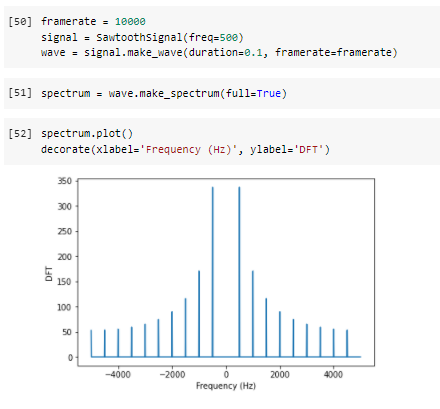
\includegraphics[width=\textwidth]{ex_1_all_work.png}
                \caption{Результаты запуска}
                \label{fig:ex_1_all_work}
            \end{figure}
            
    
    \newpage
        \section{Часть №2: Использование ДПФ}
            Во втором пункте лабораторной работы было продемонстрировано использование ДПФ (дискретное преобразование Фурье) и обратное ДПФ в виде произведения матриц. Такие операции занимают время \texttt{Nˆ2}, где \texttt{N} - длина массива, что достаточно быстро для большинства применений, но есть более быстрый алгоритм: Быстрое Преобразование Фурье (БПФ) или \texttt{FFT}, занимающий \texttt{Nlog(N)}
            
            Ключевая вещь в БПФ это лемма Даниелсона-Ланкзоса, которая предлагает рекурсивный алгоритм для DFT:
            
            \begin{enumerate}
                \item Входящий массив \texttt{y} разделяется на четное число элементов \texttt{e}, и на нечётные элементы \texttt{o}.
                \item Вычислить \texttt{DFT} \texttt{e} и \texttt{o} с помощью рекурсивных запросов.
                \item Вычислить \texttt{DFT(y)} для каждого значения \texttt{n} используя лемму Даниелсона-\\-Ланкзоса.
            \end{enumerate}

            В случае если длина исходного массива равна 1, \texttt{DFT(y) = y}. Или если длина y очень мала, можно вычислить её \texttt{DFT} с помощью матричного умножения, используя предварительно вычисленную матрицу.
            
            Начнём с небольшого реального сигнала и вычислим его БПФ:
            
             \begin{figure}[H]
                \centering
                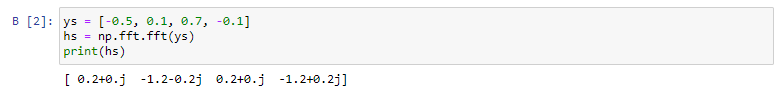
\includegraphics[width=\textwidth]{ex_2_fft.png}
                \caption{Получение БПФ}
                \label{fig:ex_2_dfr_result}
            \end{figure}
            
            Теперь нам необходимо реализовать функцию \texttt{dft} для вычисления матрицы синтеза и сразу же протестируем ее:
            
\begin{lstlisting}[language=Python, caption= Функция \texttt{dft}]
    def dft(ys):
        N = len(ys)
        ts = np.arange(N) / N
        freqs = np.arange(N)
        args = np.outer(ts, freqs)
        M = np.exp(1j * PI2 * args)
        amps = M.conj().transpose().dot(ys)
        return amps
\end{lstlisting}
            
            \begin{figure}[H]
                \centering
                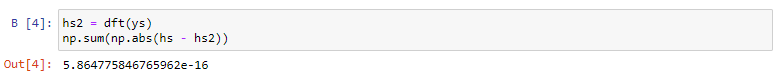
\includegraphics[width=\textwidth]{ex_2_dfr_result.png}
                \caption{Результаты работы функции \texttt{dft}}
                \label{fig:ex_2_dfr_result}
            \end{figure}
            
            После этого реализуем функцию \texttt{ff-norec}, которая будет разбивать входной массив и использовать \texttt{np.fft.fft} для вычисления БПФ половин:
            
\begin{lstlisting}[language=Python, caption= Функция \texttt{fft-norec}]
    def fft_norec(ys):
        N = len(ys)
        He = np.fft.fft(ys[::2])
        Ho = np.fft.fft(ys[1::2])
        
        ns = np.arange(N)
        W = np.exp(-1j * PI2 * ns / N)
        
        return np.tile(He, 2) + W * np.tile(Ho, 2)
\end{lstlisting}
            
            \begin{figure}[H]
                \centering
                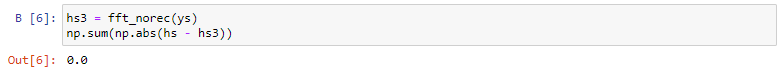
\includegraphics[width=\textwidth]{ex_2_fft_norec_result.png}
                \caption{Результаты работы функции \texttt{fft-norec}}
                \label{fig:ex_2_dfr_result}
            \end{figure}
            
            И. наконец, реализуем функцию \texttt{fft}, которая похожа на предыдущую, но \texttt{np.fft.fft} заменена на рекурсию:
            
\begin{lstlisting}[language=Python, caption= Функция \texttt{fft}]
    def fft(ys):
        N = len(ys)
        if N == 1:
            return ys
        
        He = fft(ys[::2])
        Ho = fft(ys[1::2])
        
        ns = np.arange(N)
        W = np.exp(-1j * PI2 * ns / N)
        
        return np.tile(He, 2) + W * np.tile(Ho, 2)
\end{lstlisting}
            
            \begin{figure}[H]
                \centering
                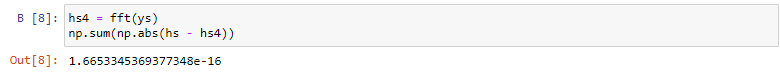
\includegraphics[width=\textwidth]{ex_2_fft_result.png}
                \caption{Результаты работы функции \texttt{fft}}
                \label{fig:ex_2_fft_result}
            \end{figure}
            
            В результате можно сказать, что полученная нами реализация БПФ занимает вермя, которое пропорционально \texttt{Nlog(N)} при создании и копировании массивова, а также занимает аналогичное количество места.
            
    \newpage
        \section{Выводы}
             В результате выполнения лабораторной работы мы изучили, что такое ДПФ, БПФ, а также создали функцию для вычисления БПФ, которая работает за \texttt{Nlog(N)} при создании и копировании массивова. Кроме того мы прошлись по всем примерам из блокнота \texttt{chap07.ipynb}, запустив все блоки кода и прочитав всю информацию.
            
\end{document}
